	
\section{Discussion}
 Oftentimes, tacit information is trapped within emails, but using \gls{JIRA} and \gls{Confluence} together will capture this information forever. In addition, \gls{Confluence} and \gls{JIRA} have permissions to give flexibility to decide who can view and edit content.
 \subsection{JIRA}
Before JIRA Microsoft SharePoint, a document management system was used to “store, organize, share, and access information” \cite{sharepoint:Online}. An issue in JIRA is used to create, track and resolve reported client issues. MOTI IMB employees use JIRA on a daily basis, so an “issue could represent a software bug, a project task, a helpdesk ticket, etc.” \cite{issueDefinition:Online}.  \\

 JIRA is highly customizable, organized by projects, components, versions and labels. The most flexible way to search for issues is by constructing JQL (JIRA Query Languages) filters that use issue fields, operators, values and keywords and return specified JIRA issues. JIRA has spilt into 3 different standalone products JIRA Core, JIRA software, and JIRA Service Desk. Designed for managing projects and tasks, JIRA Core keeps team organized. JIRA Software allows for Agile boards and integrates with software development tools.  JIRA Service Desk is IT service desk and customer service software. JIRA incorporates time tracking, reporting features and is enhanced by installing add-ons such as ScriptRunner and Tempo Timesheets. Despite regular use of JIRA at MOTI IMB, its extensive functionality and plethora of features will confuse newcomers. 
 
 \subsubsection{Overview}
 Although JIRA originated as a software tool geared towards developers, it has evolved to address the needs of the non-technical users. \gls{JIRA} can track issues, display information on a dashboard and manage \gls{agile} projects by using \gls{kanban} or \gls{scrum} Boards which are designed to manage software projects. JIRA permissions are setting that limit what users can see and do. JIRA’s permission scheme includes editing issues, creating issues, commenting, assigning issues, etc. \cite{PermissionsOverview:Online}. Generally, users are added to an JIRA project, begin searching for issues, close \gls{issue} and repeat. 
  \subsubsection{Issues}
  An \gls{issue} contains multiple fields including type, priority, component, status, resolution, description assignee and reporter. It contains information indicating the urgency and current status of the issue. Some of the options available for issue status field include new, to-do, in progress, hold, and closed. Issue priorities vary from trivial to blocker. Classifying issues correctly is essential for users to document their work and reference in the future. Issues can have subtasks, be duplicated or be related to other existing issues. Watching an issue notified the user when the issue is commented, status changed, closed, or updated.
  \begin{figure}
  	
\includegraphics[width=1\linewidth]{cloud.jpg}
  	\caption{Clouds}
  \end{figure}
 \noindent When the status of an issue is changed or closed the reporter will receive an email update. Time tracking in \gls{JIRA} is accomplished by creating a work log, entering time spent, giving a reasonable remaining estimate and description of work done. Oftentimes, issues are reassigned to assignees better suited to complete the task. Attachments can be added to the issue to better describe work that needs to be done. Previously at IMB, for each application a Microsoft \gls{sharepoint} site would be created, and issue tracking was managed by creating list items. Even though this worked for small groups, providing access to each individual SharePoint site was cumbersome and time-consuming for everybody. A single system that contains issues for all projects benefits all users and has become essential to day-to-day operations. \\ 
 
 \noindent Issues in JIRA can be imported or exported to and from xls files, which allows the user to reuse content from fabricated in other applications. Overall, JIRA issues can represent anything ranging from software bugs, to an access request and used for project management.
 
 \subsubsection{Dashboards}
 JIRA dashboards contains information boxes known as gadgets that can display dynamic data about a JIRA filter or project. Gadgets let you customize the information that appears on dashboards. Configuring dashboards allows different kinds of information to be displayed.  Most of these gadgets require JIRA filters to feed information into it. Dashboards can display filter results, issue statistics, pie charts grouped by a specified issue field such as created, assignee, status, and priority. Add-ons for JIRA should as Zephyr (used for test management) and Tempo Timesheets (creates timesheets for JIRA issues) are packaged with dashboard gadgets containing additional information specific to that add on. An example is the user timesheet add-on from tempo which displays a timesheet for a specific period of time.  \\ 
 \begin{figure}
 	
\includegraphics[width=1\linewidth]{data1.jpg}
 	\caption{People}
 \end{figure}

At this time, dashboard usage is inconsistent, and undergoing further investigation. Ideally, every project and every team would have a JIRA dashboard, customized to suit their individual needs.  

Also, \gls{JIRA} has adaptable \gls{kanban} and \gls{scrum} boards to track issue backlogs. These boards can be displayed on a JIRA dashboard. Creating a meaningful dashboards faces several obstacles including understanding of the JIRA specific query language, \gls{jql}, knowledge of which dashboard gadget is suitable and a steep learning curve.  \\

Developing an informative \gls{JIRA} dashboard entails consulting with the end users, multiple iterations and producing JIRA filters.

 \begin{figure}
	
\includegraphics[width=1\linewidth]{datavisual.png}
	\caption{Visuallizing Data}
 \end{figure}

Dashboards are the best method to visually reporting on ongoing and completed issues in \gls{JIRA}.

\subsubsection{Agile Projects in JIRA}
Agile software development is used by the PEOPLE to produce software that better suits the needs of customers. 
In \gls{agile}, requirements and solutions develop through frequent conversations with stakeholders as software is developed through collaboration. Two kinds of agile boards are available in JIRA Agile, Kanban and Scrum. Each of these boards are designed to follow their specific agile methodology. Adding the fix version field to an issue will assign it to a particular release. All released and unreleased versions can be viewed within the project sidebar in JIRA. JIRA software provides tools specifically for any agile project management which include boards, releases and dashboard gadgets (burndown charts, velocity charts and more).

\begin{figure}
	
\includegraphics[width=1\linewidth]{q.jpg}
	\caption{Typical Pictures}
\end{figure}

\begin{table}
	\caption{Time log for ELEC 360 --- Assignment 2}
	\begin{tabular}{c c c c c}
		Week of Oct 8 &                 Week of Oct 15 &                      Week of Oct 22 &                                    Week of Nov 5 &                             Week of Nov 12 \\
		5 hours Prepared for ELEC 360 Lab and completed it &  2 hours working on lab report &  3 hours spent on preparing for lab &  3 hours doing the prelab and and lab experiment &  2 hours working on lab report \\
		3 hours of studying for quizzes &  3 hours studying for midterm &  2 hours studying midterm solutions &  2 hours reviewing for quizzes &  5 hours solving question for assignment 2 \\
		1 hour creating notes &  2 hours preparing for midterm &  2 hours preparing for quizzes &  3 hours solving questions of assignment 2 &  1 hour studying for quizzes \\
	\end{tabular}
\end{table}

Altogether, JIRA is well-suited for \gls{agile} project management with boards, versioning and dashboard gadgets.  

\subsubsection{Add-ons}
JIRA add-ons provide additional functionality to JIRA including increased customization and features. 

Adaptavist ScriptRunner provides custom workflows, custom JQL and executes scripts that interact with JIRA. Some notable features include custom automatic emails triggered when an issue transitions into a particular state, enhanced JIRA filters (i.e. searching for issues attachments) and adding additional fields for JIRA issues. This add-on provides a simple way to script in JIRA. \\ 

\noindent Tempo timesheets enhances time tracking and reporting features while faultlessly integrating with JIRA. It helps teams and managers track time, be efficient and used for forecasting. This add-on is useful because it allows JIRA users to accurate track their time spent on issues, projects and make strategic decisions based on this info. \\
The tempo time tracker runs within JIRA and is the best way track time.

\begin{figure}
	\centering
	
\includegraphics[width=0.4\textwidth,keepaspectratio]{final.jpg}
	\caption{Final Pictures}
\end{figure}

A user timesheet contains information about hours worked, planned, and required for the week. It organizes issues automatically organizes issues by project and component.

\begin{figure}
	\centering
	
\includegraphics[width=1\textwidth,keepaspectratio]{n.jpg}
	\caption{Cool Looking USBs.}
\end{figure}

\subsubsection{Limitations}
JIRA can be extremely slow at times which may be caused by running out of memory, and a large JIRA instance \cite{issues:Online}. Extensive functionality such as time tracking, \gls{agile} boards, dashboards and user timesheets are underutilised because users unaccustomed to JIRA. Additionally, a lack of tutorials or instructions are how to use JIRA compound the difficult of learning how to use \gls{JIRA}. 

\subsection {Confluence}
\gls{Confluence} is team-based collaboration software developed by Atlassian used at the ORGANIZATION to document projects and work in conjunction with \gls{JIRA}. Confluence works by It organizes content by labels, can embed videos on pages and is highly customizable. The aim of Confluence is to become the tool for organizing, discussing, and doing work. Assigning tasks, recording meeting notes and sharing documents are some of the features of Confluence.
\subsubsection{Overview}
Confluence keeps page and file versions to track every version of documents. Despite numerous free wiki-software available on the web, Confluence has page hierarchy (page trees), transparency when creating content and clean user interface which make it suitable for documentation.
\subsubsection{Spaces}
Everything in Confluence is organized in spaces, which are a collection of related pages. Pages are the documents in which the team will create, edit, and discuss work. Confluence Spaces are organized by categories (i.e., critical non-critical, documentation and software-project). Spaces can be customized to fit the need of each team. For example uses of Confluence include knowledge bases, technical documentation and organizing content \cite{confluence:Online}.
\subsubsection{Pages}
In a Confluence page, content is created, collected, and accessed in one place.

\begin{figure}
	\centering
	
\includegraphics[width=0.8\textwidth,keepaspectratio]{l.jpg}
	\caption{Creating Life}
\end{figure}

\noindent \gls{Confluence} pages contain text, images, videos and uses macros that add extra functionality or include dynamic content. Macros can create charts, incorporate existing Microsoft documents (Word, Excel, PowerPoint) and reuse content on Confluence pages. Existing templates in Confluence serve as an excellent starting point for users to start creating documentation for Confluence. Customizing page and space templates is an essential feature to save time and reuse content.

\subsubsection{Embedding Content}
Attachments are useful for sharing existing content saved in a different file format. 
\begin{figure}
	\centering
	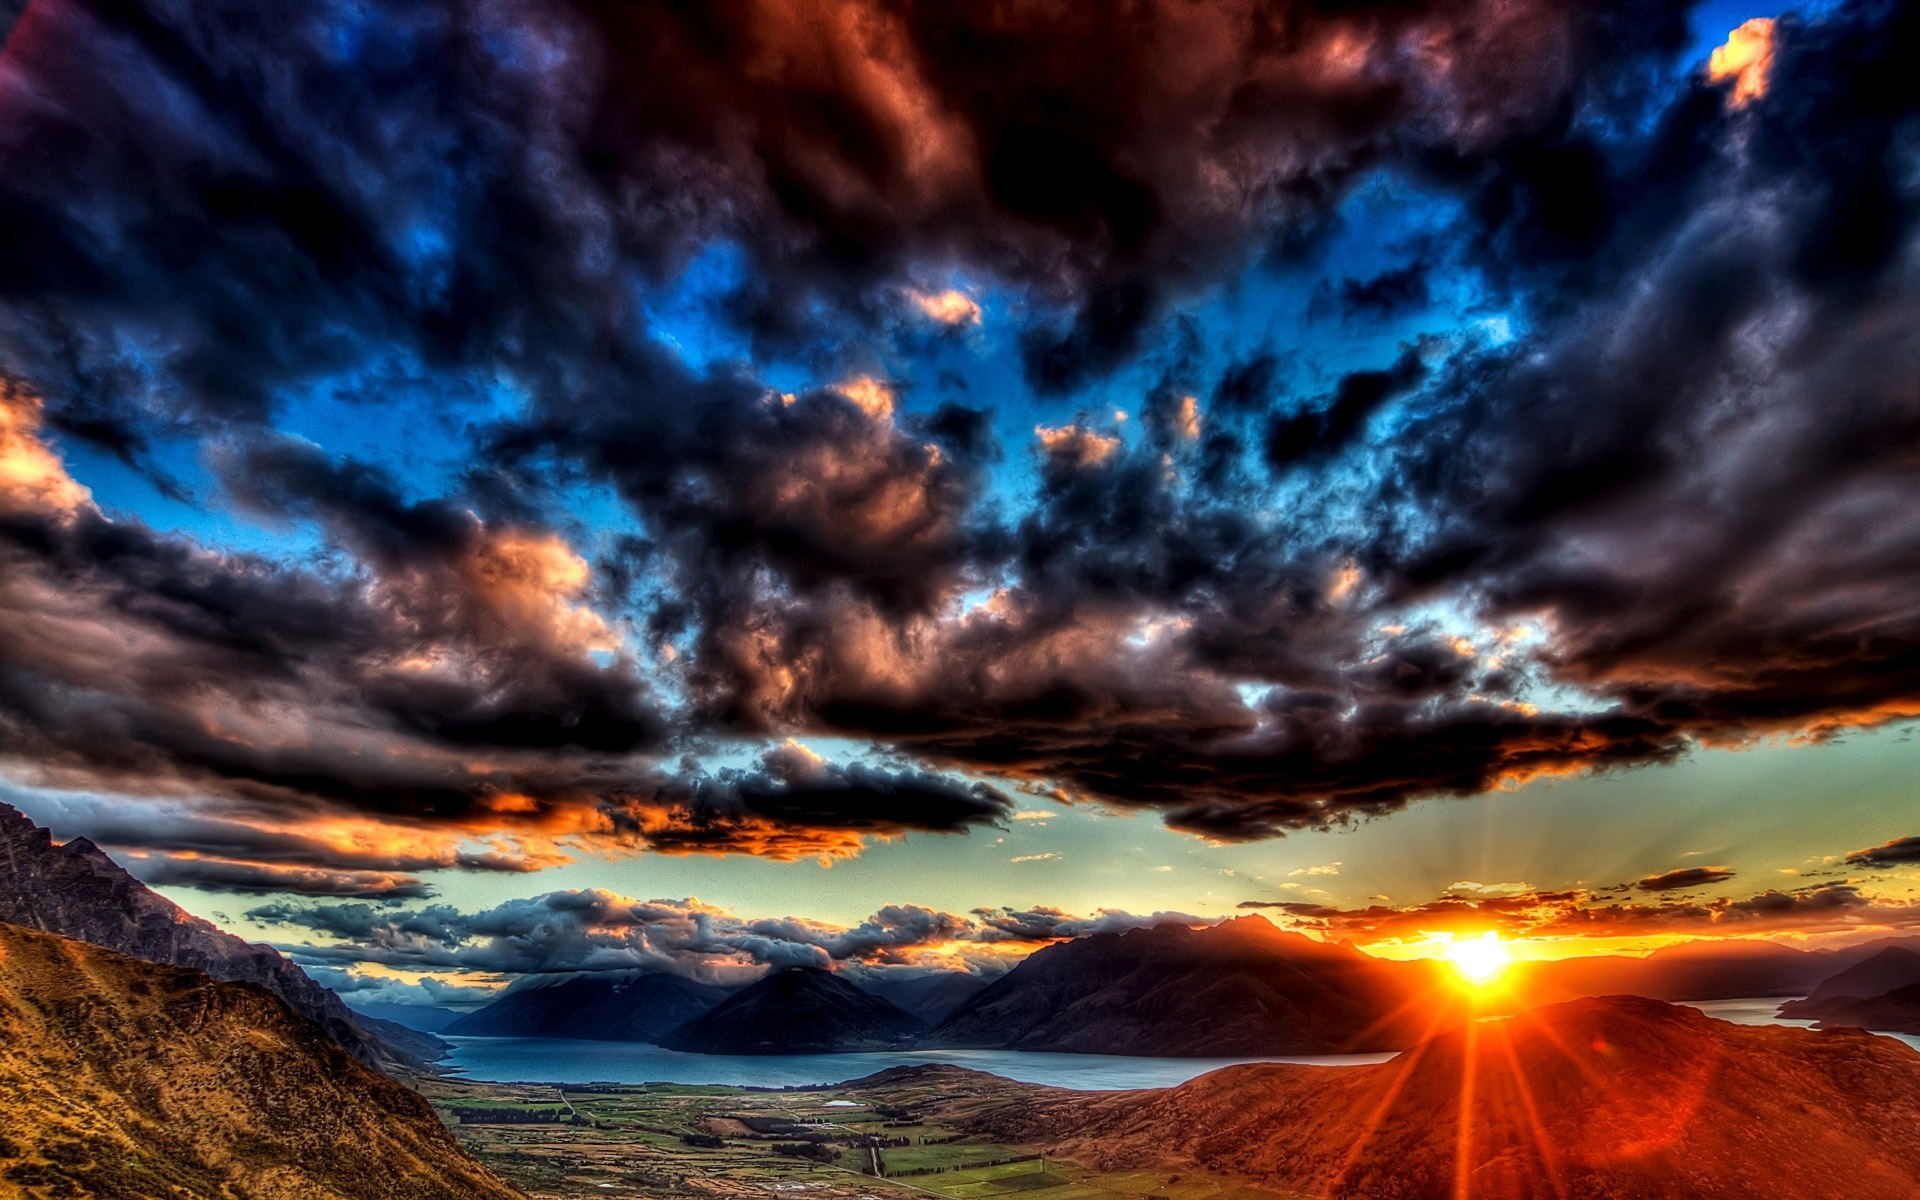
\includegraphics[width=0.5\textwidth,keepaspectratio]{good.jpg}
	\caption{Good Picture}
\end{figure} 
When word documents imported into Confluence, that document's content is copied onto one or more Confluence pages. Additionally, images and videos from the web can be embedded into a Confluence Page. Sharing links is convenient and helps users find information.

\subsubsection{Limitations}
Confluence is designed for documentation, used by large organizations including NASA \cite{NASA:Online}, yet documenting legacy and current projects in Confluence is not occurring at this moment. Currently, use of Confluence is limited to few internal users, so education about this software and its functionality lacking. Certain files types such as mpp (Microsoft Project) and vsd (Microsoft Visio) cannot be embedded within a Confluence Page, but can be uploaded as a file.  Creating structured space templates and pages will allow content to be streamlined. Confluence functionality can be extending by downloading add-on in the Atlassian marketplace. For example, tables in Confluence are rudimentary, consisting only of ascending/descending sorting, however, a few add-ons for Confluence address this problem.

\subsection{JIRA and Confluence Integration}
Much like how Microsoft Office Products integrate well together, JIRA and Confluence are better together. When \gls{Confluence} and JIRA sites are connected JIRA issues can be created, viewed and more from within Confluence. Also, connecting JIRA with Confluence allows pie charts, created vs resolved chart and filter results etc.  Essentially, existing information stored in JIRA can be reported in Confluence by the JIRA issues macro or the JIRA charts macro \cite{JAC:Online}.

\noindent Another benefit from connecting JIRA to \gls{Confluence} is delegated user management to \gls{JIRA}, so all users can be managed in a single location. Whenever a link is created to a JIRA issue in Confluence, or link to a Confluence page from a JIRA application, the JIRA Links button appears at the top of the Confluence page. This makes it very simple to jump from JIRA straight into Confluence and vice-versa.
\begin{figure}
	\centering
	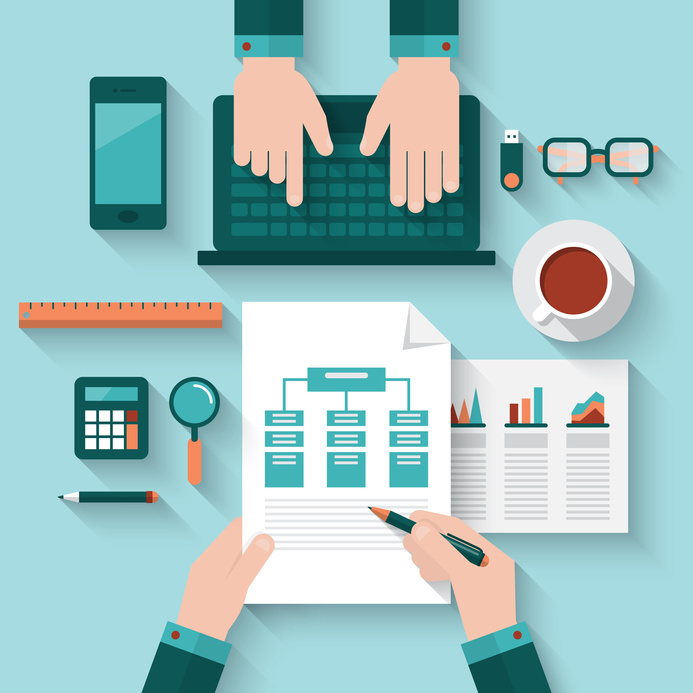
\includegraphics[width=0.5\textwidth,keepaspectratio]{goddata.jpg}
	\caption{Good Looking Report}
\end{figure} 
\noindent The tight integration between Confluence and JIRA results in related issues can be accessed directly from the Confluence page with their current status.